\chapter{Higgs Mekanizması}
\lhead{\emph{Kütle Terimi ve Kendiliğinden Simetri Bozulması}} 
\section{Kütle Terimi ve Kendiliğinden Simetri Bozulması}
Bu bölümde Higgs mekanizmasının neden gerekli olduğu ve Higgs mekanizmasının anlaşılması öncü olacak adımlar belirtilecektir. Öncelikle Higgs mekanizması $W^{+},W^{-}$ ve $Z^{0}$ bozonlarına kütle kazandıramadığımızdan ihtiyacımız olmaktadır. Bu bozonların kütle kazanma mekanizmasına benzer şekilde diğer temel parçacıkların kütle kazanılması açıklanabilmektedir. Standart Model teorimizi renormalize edilebilir olmasını sağlamak için model içerisinde yüksek dereceli alan terimlerini sağlayacak olan ifadeler içermesi gerekmektedir. Bu bize Feynman diyagramları hesaplamalarında olduğu gibi bazı sonlu çıkacak ifadelerin sonsuz çıkması halinde sonsuzluk ifadelerinden kurtulabilmenin yolunu sunabilmesinde yararlıdır. Öncelikle skaler $\phi$ alanı için Lagranjiyeni
\begin{equation} \label{ksb1}
\mathcal{L} = \frac{1}{2}(\partial_{\mu}\phi)(\partial^{\mu}\phi) + e^{(\alpha\phi)^{2}}\qquad(\alpha\;\textrm{gerçek bir sabit olmak üzere})
\end{equation}
olarak verelim. Buradaki üstel terimi seriye açtığımızda
\begin{equation} \label{ksb2}
\mathcal{L} = \underbrace{ \frac{1}{2}(\partial_{\mu}\phi)(\partial^{\mu}\phi)}_{\textrm{Kinetik terim}} +  \underbrace{1}_{\textrm{Sabit}} + \underbrace{ \alpha^{2}\phi^{2}}_{\textrm{Kütle terimi}} + \underbrace{ \frac{1}{2}\alpha^{4}\phi^{4} + \frac{1}{6}\alpha^{6}\phi^{6} + \cdots }_{\textrm{Yüksek mertebe terimler}}
\end{equation}
ele ederiz. Bu ifadeyi bir kalıba oturtabilmek için
\begin{equation} \label{ksb3}
\mathcal{L}_{K-G} = \frac{1}{2}(\partial_{\mu}\phi)(\partial^{\mu}\phi) - \frac{1}{2}\left(\frac{m_{K-G}\,c}{\hbar}\right)^{2} \phi^{2}
\end{equation}
%\qquad \left(\textrm{kütle terimi = } \frac{1}{2}\left(\frac{mc}{\hbar}\right)^{2} \right)
olan Klein-Gordon Lagranjiyenine bakalım.	Klein-Gordon Lagranjiyenindeki kütle terimi ifadesi önündeki işaret negatiftir ve denklem \eqref{ksb2}'e baktığımızda eğer
$$
\alpha^{2} < 0 \qquad m_{K-G} = \sqrt{2}\frac{\alpha\, \hbar}{c}
$$ 
kabullerini yaparsak düzgün işaretli kütle terimi ve real kütle ifademizi elde etmiş oluruz. Bu bilgiler ışığında
$$
\mathcal{L} = \underbrace{\frac{1}{2}(\partial_{\mu}\phi)(\partial^{\mu}\phi)}_{\textrm{Kinetik Terim}} - \underbrace{ V(\phi)}_{\textrm{Potansiyel Terimi}}
$$
genel Lagranjiyen ifademizi yazarak başlayalım. Potansiyel terim için
$$
V(\phi) = \frac{1}{2} \mu^{2}\,\phi^{2} + \frac{1}{4}\lambda\phi^{4}
$$
ifadesini kullanırsak
\begin{equation} \label{ksb4}
\mathcal{L} = \frac{1}{2}(\partial_{\mu}\phi)(\partial^{\mu}\phi) - \frac{1}{2} \mu^{2}\,\phi^{2} - \frac{1}{4}\lambda\phi^{4}
\end{equation}
olarak belirtilen Lagranjiyeni elde ederiz. Bu skaler alan için Lagranjiyen ifadesi $\phi \to -\phi$ dönüşümü altında simetriktir ve Lagranjiyen ifadesinde mutlak minimum değerini sağlayabilmek için yada diğer bir değişle Hamiltonyenin bağlı olmasını kesinleştirmek için $\lambda > 0$ olarak seçilmektedir. Feynman cebirine göre  taban durumdan "vakum" başlayarak küçük  pertürbasyonlar uygularız ve alanları taban durumu etrafındaki salınımlar olarak ele alırız. Daha önceleri kullandığımız alanlar olan Klein-Gordon ($\phi$), Dirac ($\psi$) ve Vektör ($A^{\mu}$) alanlarının taban durumları sıfırdır ve bu alanları sıfır noktası etrafındaki salınımlar olarak ele alınmaktadır. İlk olarak Denklem \eqref{ksb4}'deki Lagranjiyen ile tasvir edilen alanın minimum değeri
\begin{equation} \label{ksb5}
\frac{d V(\phi)}{d\phi} = 0\qquad \to \qquad \phi_{0}(\mu^{2} + \lambda\phi_{0}^{2}) = 0
\end{equation}
ifadesi kullanılarak bulunur. Bu minimum fonksiyonunda $\mu^{2} > 0$ (bu durumu $\mu_{+}^{2}$ olarak) ve $\mu^{2} < 0$ (bu durumu $\mu_{-}^{2}$ olarak) durumlarını inceleyelim. Minimum değerlerini elde etmek için öncelikle $\mu_{+}^{2} > 0$ durumunu incelediğimizde $\phi_{0} = 0$ değerinde bir vakum değeri olmaktadır. Fakat $\mu_{-}^{2}$ durumu için 
\begin{equation} \label{ksb6}
\phi^{+}_{0} = + \sqrt{\frac{- \mu^{2}_{-} }{\lambda}} = +v \qquad \textrm{ve} \qquad
\phi^{-}_{0} = - \sqrt{\frac{- \mu^{2}_{-} }{\lambda}} = -v 
\end{equation}
vakum beklenen değerlerini elde ederiz.  $\mu_{-}^{2}$ seçimi biraz garip gözükmektedir, çünkü bize sanal kütleye sahip bir parçacığı anlatıyor gibi gelebilir. Fakat bu durumda parçacığın $\phi_{0} = 0$ değeri için pertürbasyon teorisini uyguladığımızda bu nokta kararlı bir minimum olmadığından şimdilik bir anlam taşımaz.
\begin{figure}
\begin{minipage}{\linewidth}
      \centering
      \begin{minipage}{0.45\linewidth}
          \begin{figure}[H]
              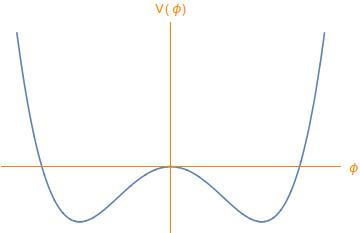
\includegraphics[width=\linewidth]{higgs}
              \caption{$\mu^{2} > 0$ için}
          \end{figure}
      \end{minipage}
      \hspace{0.05\linewidth}
      \begin{minipage}{0.45\linewidth}
          \begin{figure}[H]
              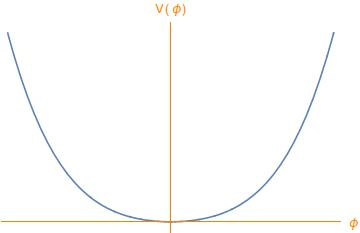
\includegraphics[width=\linewidth]{higgs2}
              \caption{$\mu^{2} < 0$ için}
          \end{figure}
      \end{minipage}
  \end{minipage}
  \caption{Potansiyel $V(\phi)$ fonksiyonu grafikleri.}
  \label{higgspot}
\end{figure}
Vakum değeri etrafında küçük pertürbasyonlar uygulamamız gerektiğinden $+v$ veya $-v$ beklenen  değerlerinden birini seçmek durumunda kalırız ve yapılan herhangi bir seçimin fiziksel sonuçları aynı olacaktır. Dolayısıyla $\phi$ alanı $\eta = \phi - v$ değeri kadar kaydırılırsa ve denklem \eqref{ksb4}'deki Lagranjiyene uygulanırsa
\begin{equation} \label{ksb7}
\begin{split}
\mathcal{L} & = \frac{1}{2} (\partial_{\mu}\eta\partial^{\mu}\eta) - \frac{1}{2}\mu_{-}^{2} \left[ \eta^{2} + 2\eta v + v^2 \right] + \frac{1}{4}\lambda \left[ \eta^{4} + 4 \eta^{3} v + 6 \eta^{2} v^{2} + 4 \eta v^{3} + v^{4 } \right] \\
 & = \frac{1}{2} (\partial_{\mu}\eta\partial^{\mu}\eta) - \lambda v^{2} \eta^{2}  + \lambda v \eta^{3} + \frac{1}{4} \lambda \eta^{4} - \frac{1}{4} \lambda v^4
\end{split}
\end{equation}
ifadesi elde edilmektedir. Buradaki $\lambda v^{2} \eta^{2}$ kütle terimi ifadesi olduğundan Klein-Gordon denkleminde belirtiğimiz üzere 
\begin{equation} \label{ksb8}
\frac{1}{2} m_{\eta}^2 = \lambda v^{2} \eta^{2} \Rightarrow m_{\eta} = \sqrt{2 \lambda v^2} \qquad \textrm{ve}\quad m_{\eta} = \sqrt{-2\mu_{-}^2} 
\end{equation}
olarak $m_{\eta}$ real ve pozitif bir kütleyi göstermektir. Lagranjiyen ifademiz her ne kadar $\phi$ yerine $\eta$ olarak temsil edilse de denklem \eqref{ksb7} ve denklem \eqref{ksb4} aynı fiziksel sistemi belirtmektedir. Dikkat çekici nokta ise Lagranjiyen ifademizde $\lambda v \eta^{3}$ olan bir terim ortaya çıktı ve bu terim nedeniyle artık Lagranjiyenimiz daha öncesinde sahip olduğu $\phi \to -\phi$ kesikli simetriye (vakum beklenen değerleri $+v$ ve $-v$ 'den başka değerler almadığı için ) $\eta \to -\eta$ olarak sahip değildir. Bu durum dışardan herhangi bir müdahele olmadan ortaya çıktığından "kendiliğinden simetri kırılması" olarak adlandırılır. 

\section{Global Simetrinin Bozulması}
Bu bölümde sürekli simetrinin bozulması incelenecektir. Öncelikle kendi kendine etkileşim halinde olan yüklü bir skaler alan için Lagranjiyen ifadesi
\begin{equation} \label{gs1}
\mathcal{L} = \left( \partial_{\mu} \phi \right)^{*} \left( \partial^{\mu} \phi \right) - V (\phi^{*}\phi) \quad \textrm{ve} \qquad \phi = \frac{\phi_{1}+i \phi_{2}}{\sqrt{2}}
\end{equation}
olarak yazılabilir. Potansiyel fonksiyonu olarak da 
$$
V(\phi^{*}\phi) = \mu^{2}(\phi^{*}\phi) + \lambda (\phi^{*}\phi)^2
$$
ifadesini aldığımızda ve $\phi = \frac{\phi_{1}+i \phi_{2}}{\sqrt{2}}$ ile belirtilen alanı Lagranjiyende yerine yazar ve düzenlersek
\begin{equation} \label{gs2}
\mathcal{L} = \frac{1}{2} \left(\partial_{\mu} \phi_{1} \right)^{2} + \frac{1}{2} \left(\partial_{\mu} \phi_{2} \right)^{2} - \frac{1}{2} \mu^{2} \left( \phi_{1}^{2} + \phi_{2}^{2} \right) - \frac{1}{4} \lambda \left( \phi_{1}^{2} + \phi_{2}^{2} \right)^{2}
\end{equation}
ifadesini elde ederiz. Bu ifade Global U(1) simetrisine sahiptir. Bunu görebilmek için $\phi^{'} \to e^{i\theta}\phi$ ve $(\phi^{*})^{'} \to e^{-i\theta}\phi^{*}$ olarak ele alındığında $\phi_{1}$ ve $\phi_{2}$ uzayında dönmeler altında değişmezdir. Bu Lagranjiyen için vakum beklenen değerleri daha önce yapıldığı üzere $\mu > 0$ ($\mu_{+}$ olarak) ve $\mu < 0$ ($\mu_{-}$ olarak) durumlarını inceleyelim. Vakum beklenen değerlerini bulabilmek için öncelikle potansiyelin minimum denklemi
\begin{equation} \label{gs3}
\begin{split}
\frac{\partial V(\phi_{1},\phi_{2})}{\partial \phi_{1}} = 0 \qquad \textrm{ve} \qquad \frac{\partial V(\phi_{1},\phi_{2})}{\partial \phi_{2}}  = 0 \\
\\
\left( \phi_{1\, min} +\phi_{2\, min} \right) \left[ \mu^{2} + \lambda \left( \phi_{1 \,min}^{2} + \phi_{2 \,min}^{2} \right) \right] = 0 
\end{split}
\end{equation}
şeklinde ifade edilir. Öncelikle $\mu_{+}$ durumunu incelediğimizda sadece $\phi_{1 \,min} = 0$ ve $ \phi_{2 \,min} = 0$ vakum beklenen değeri elde edilir. Bu nokta daha önce bahsedildiği gibi kararsız bir minimum olduğundan, Feynman cebiri uygulandığında ıraksayan ifadeler elde edilir. Dolayısıyla $\mu_{-}$ durumuna baktığımızda 
$$
\mu^{2}_{-} + \lambda \left( \phi_{1 \,min}^{2} + \phi_{2 \,min}^{2} \right) = 0 \quad \Rightarrow \quad  \sqrt{ \phi_{1 \,min}^{2} + \phi_{2 \,min}^{2} }  = \sqrt{ \frac{- \mu_{-}^{2}}{\lambda} } = v
$$
Bu çember denklemini sağlayan sonsuz sayıda $\phi_{1 \,min}$ ve $\phi_{2 \,min}$ değerleri olması sürekli bir simetriyi oluşturmaktadır. Feynman cebirini uygulayabilmek için çember üzerindeki $\phi_{1 \, min} = v$ ve $\phi_{2 \, min} = 0$ ayarlarını seçtiğimizde
$$
\eta = \phi_{1} - v \quad \textrm{ve} \quad \xi = \phi_{2} \quad \Rightarrow \quad \phi = \frac{ ( \eta + v ) + i \xi }{\sqrt{2}}
$$ 
ve Lagranjiyende yerlerine koyduğumuzda 
\begin{equation} \label{gs4}
\begin{aligned}
\mathcal{L} (\eta \,, \xi) &= \frac{1}{2} \left(\partial_{\mu} \eta \right)^{2} + \frac{1}{2} \left(\partial_{\mu} \xi \right)^{2} - \underbrace{\lambda v^{2} \eta^{2}}_{\eta\; \textrm{kütle terimi}} - \underbrace{0\, \xi^{2}}_{\xi \; \textrm{kütle terimi}} \\
\\
& - \underbrace{ \frac{1}{4} \lambda \eta^{2} - \lambda v \eta^{3} - \frac{1}{2} \lambda \eta^{2} \xi^{2} - \lambda v \eta \xi^{2} - \frac{1}{4} \lambda \xi^{4} }_{\textrm{Etkileşim terimleri}} - \underbrace{\frac{1}{4} \lambda v^{4}}_{\textrm{Sabit terim}}
\end{aligned}
\end{equation}
ifadeleri ortaya çıkmaktadır. Lagranjiyendeki $\eta$ ve $\xi$ alanlarının kütleleri olarak
\begin{equation} \label{gs5}
\frac{1}{2} m_{\eta}^{2} = \lambda v^2 \to  m_{\eta} = \sqrt{- 2 \mu^{2}_{-}} \quad m_{\eta} > 0 \quad ve \quad m_{\xi} = 0
\end{equation}
yazılabilir. Çember üzerindeki özel minimum noktaları seçtiğimizden dolayı sistemin sahip olduğu simetri bozulduğu için elde edilen Lagranjiyende $\xi$ alanı kütlesi $m_{\xi} = 0$  bir skaler alan olarak ortaya çıkmaktadır. Goldstone teoremine göre global bir simetrinin kendiğiliğinden bozulması sonucu olarak bir spin-0 kütlesiz parçacığın oluştuğunu söylemesiyle bu durumu açıklayabiliriz. Fakat bilinen parçacıkların listesinde böyle bir bozon yoktur. Dolayısla zayıf etkileşme bozonlarına kütle kazandırabilmek için teorimizde başka bir simetriyi ele almamız gereklidir.

\lhead{\emph{Abelyan Higgs Mekanizması}} 
\section{Abelyan Higgs Mekanizması}
Önceki bölümlerde yerel ayar dönüşümü altında Lagranjiyende kinetik enerji terimindeki türev işlemcisinden dolayı teorimizde foton alanı için bir kütle terimi meydana gelmişti. Teorimizi yerel ayar dönüşümü altında değişmez bırakmak istediğimizden fotonu belirten vektör alanının kütle terimini ortadan kaldırmıştık. Bu bölümde zayıf etkileşmeler için kütle terimini getirebilmek için önceki yapılanların eşliğinde bu yola başvuracağız. Lagranjiyen ifademizi
\begin{equation} \label{abe1}
\mathcal{L} = \left( \partial_{\mu} \phi \right)^{*} \left( \partial^{\mu} \phi \right) - \mu^{2}(\phi^{*}\phi) - \lambda (\phi^{*}\phi)^2 \quad \textrm{ve} \qquad \phi = \frac{\phi_{1}+i \phi_{2}}{\sqrt{2}}
\end{equation}
olarak yazalım. Yerel ayar dönüşümü için
\begin{equation} \label{abe2}
\partial_{u} \to \mathcal{D}_{\mu} = \partial_{\mu} - i \frac{q}{\hbar c} A_{\mu} \qquad \textrm{ve} \qquad A^{'}_{\mu} \to A_{\mu} + \partial_{\mu} \alpha(x)
\end{equation} 
ifadelerini kullanacağız. Burada kovaryant türev ifadesi ile eklenen  $A_{\mu} $ alanı için serbest Lagranjiyen ifadesi de eklendiğinde
$$
\mathcal{L} = \left( \mathcal{D}_{\mu} \phi \right)^{*}  \left( \mathcal{D}^{\mu} \phi \right) - \frac{1}{4} F^{\mu \nu} F_{\mu \nu} - \frac{1}{2} \mu^{2} \left( \phi_{1}^{2} + \phi_{2}^{2} \right) - \frac{1}{4} \lambda \left( \phi_{1}^{2} + \phi_{2}^{2} \right)^{2}	
$$
elde edilmektedir. Bu Lagranjiyeni daha açık bir şekilde yazarsak
\begin{equation} \label{abe3}
\begin{aligned}
\mathcal{L} &= \left[ \left( \partial_{\mu} + \frac{i\,q}{\hbar \, c} A_{\mu} \right) \left(\frac{\phi_{1} - i \phi_{2}}{\sqrt{2}} \right) \right] \left[ \left( \partial^{\mu} - \frac{i\,q}{\hbar \, c} A^{\mu} \right) \left(\frac{\phi_{1} + i \phi_{2}}{\sqrt{2}} \right) \right] \\
\\
& - \frac{1}{4} F^{\mu \nu} F_{\mu \nu} - \frac{1}{2} \mu^{2} \left( \phi_{1}^{2} + \phi_{2}^{2} \right) - \frac{1}{4} \lambda \left( \phi_{1}^{2} + \phi_{2}^{2} \right)^{2}
\end{aligned}
\end{equation}
elde edilir. Bu ifade de sadece kinetik enerji terimini düzenlediğimizde
\begin{equation} \label{abe4}
\begin{aligned}
\mathcal{L}_{Kinetik} &= \left[ \frac{1}{\sqrt{2}} \left( \partial_{\mu} \phi_{1} \right)
 - \frac{i}{\sqrt{2}} \left( \partial_{\mu} \phi_{2}  \right) + 
 \frac{i q}{\sqrt{2}\,\hbar c} \left( A_{\mu} \phi_{1} \right) +
 \frac{q }{\sqrt{2}\,\hbar c} \left( A_{\mu} \phi_{2} \right) \right] \\
 \\
 &\quad\, \left[ \frac{1}{\sqrt{2}} \left( \partial^{\mu} \phi_{1} \right)
 + \frac{i}{\sqrt{2}} \left( \partial^{\mu} \phi_{2}  \right) - 
 \frac{i q}{\sqrt{2}\,\hbar c} \left( A^{\mu} \phi_{1} \right) +
 \frac{q }{\sqrt{2}\,\hbar c} \left( A^{\mu} \phi_{2} \right) \right] \\
 \\
 &= \frac{1}{2} \left( \partial_{\mu} \phi_{1} \right)^{2} +
 \frac{1}{2} \left( \partial_{\mu} \phi_{2} \right)^{2} + 
 \frac{1}{2} \left(\frac{q}{\hbar \, c} \right)^{2} \left( \phi_{1}^{2} + \phi_{2}^{2} \right) A_{\mu} A^{\mu}\, \\
 \\
 & + \frac{q}{\hbar \, c} \bigg\lbrace  \left( \partial_{\mu}\phi_{1} \right)\phi_{2} - \left( \partial_{\mu}\phi_{2} \right) \phi_{1} \bigg\rbrace A^{\mu}
\end{aligned}
\end{equation}
olarak elde edilmektedir. Bir önceki bölümde yaptığımız gibi $\mu > 0$ ($\mu_{+}$ olarak) ve $\mu < 0$ ($\mu_{-}$ olarak) durumlarının sonuçlarını bildiğimizden vakum beklenen değeri için  $\mu_{-}$ durumunu ele alacağız ve bu bize minimumlar çemberi $$\sqrt{ \phi_{1 \,min}^{2} + \phi_{2 \,min}^{2} }  = \sqrt{ \frac{- \mu_{-}^{2}}{\lambda} } = v $$
ifadesini belirtecektir. Önceki bölümdeki gibi 
$$
\eta = \phi_{1} - v \quad \textrm{ve} \quad \xi = \phi_{2} \quad \Rightarrow \quad \phi = \frac{ ( \eta + v ) + i \xi }{\sqrt{2}}
$$ 
minimum değerleri seçildiğinde denklem \eqref{abe7}
\begin{equation*}
\begin{aligned}
\mathcal{L} &= \frac{1}{2} \left( \partial_{\mu} \eta \right)^{2} +
 \frac{1}{2} \left( \partial_{\mu} \xi \right)^{2} + 
 \frac{1}{2} \left(\frac{q}{\hbar \, c} \right)^{2} \left( (\eta + v)^{2} + \xi^{2} \right) A_{\mu} A^{\mu}\, \\
 \\
 & + \frac{q}{\hbar \, c} \bigg\lbrace  \left( \partial_{\mu} \eta  \right)\xi - \left( \partial_{\mu}\xi \right) (\eta + v) \bigg\rbrace A^{\mu}  - \lambda v^{2} \eta^{2} - 0\, \xi^{2} \\
 \\
& - \frac{1}{4} \lambda \eta^{2} -  \lambda v \eta^{3} - \frac{1}{2} \lambda \eta^{2} \xi^{2} - \lambda v \eta \xi^{2} - \frac{1}{4} \lambda \xi^{4}  - \frac{1}{4} \lambda v^{4}
 \end{aligned}
\end{equation*}
haline gelmektedir ve ifadeler düzenlendiğinde
\begin{equation} \label{abe5}
\begin{aligned}
\mathcal{L} &= \left[ \frac{1}{2} \left( \partial_{\mu} \eta \right)^{2} - \lambda v^{2} \eta^{2} \right] + 
 \left[ \frac{1}{2} \left( \partial_{\mu} \xi \right)^{2} -  0\, \xi^{2} \right]  \\
 \\
 & + \left[ - \frac{1}{4} F^{\mu \nu} F_{\mu \nu} + \frac{1}{2} \left( \frac{q}{\hbar \, c}\right)^2 v^{2} A_{\mu} A^{\mu} \right] \\  
 \\
 & + \left[ \frac{q}{\hbar \, c} \left\lbrace \left( \partial_{\mu} \eta \right) \xi - \left( \partial_{\mu} \xi \right) \eta - v \left( \partial_{\mu} \xi \right) \right\rbrace A^{\mu} \right] \\
 \\
 & + \left[ \left( \frac{q}{ \hbar \, c} \right)^{2} v \eta A_{\mu} A^{\mu} +
  \frac{1}{2} \left( \frac{q}{ \hbar \, c} \right)^{2} \left\lbrace \eta^{2} + \xi^{2} \right\rbrace A_{\mu} A^{\mu} \right] \\
  \\
 & + \left[ - \frac{1}{4} \lambda \eta^{2} -  \lambda v \eta^{3} - \frac{1}{2} \lambda \eta^{2} \xi^{2} - \lambda v \eta \xi^{2} - \frac{1}{4} \lambda \xi^{4} \right]  + \frac{1}{4} \lambda v^{4}
\end{aligned}
\end{equation}
Lagranjiyeni elde edilmektedir. Bu Lagranjiyende $\xi$ alanı kütlesiz ($m_{\xi} = 0$) spin-0 Goldstone bozonu olarak ortaya çıkmakta ve kütle kazanmış bir vektör alanı $A^{\mu}$ 
\begin{equation} \label{abe6}
\frac{1}{2}m_{A}^{2} =  \frac{1}{2} \left( \frac{q}{\hbar \, c}\right)^2 v^{2}  \quad \to \quad m_{A} = \frac{q}{\hbar \, c} v
\end{equation}
ifadesi (Proca Lagranjiyeni ifadesine benzer şekilde) meydana gelmektedir. Fakat kolayca yorumlanamaycak
$$
\frac{q}{\hbar \, c} v \, \left(\partial_{\mu}\xi \right) A^{\mu}
$$
terimi bulunmaktadır. Dolayısıyla bir şekilde $\xi$ alanında kurtulmanın yolunu bulmamız gerekir. Bunu sağlamak üzere öncelikle   vakum durumu etrafında küçük dalgalanmalar olarak betimleyebilmek için alanımızı  $\phi$'yi polar koordinatlarda
\begin{equation} \label{abe7}
\phi(x) = \frac{1}{\sqrt{2}} \left( \eta (x) + v \right) e^{i \frac{\xi (x)}{v}}
\end{equation}
olarak yazarız. Burada yerel olarak bir ayar dönüşümü yaparak $\phi$ alanının fazını sadece real kısımı kalacak şekilde $\xi$ alanını ortadan kaldırabiliriz. Bunu yapabilmek için $\alpha(x) = - \frac{\xi (x)}{v} $ olarak adlandıralan birimsel ayarı seçeriz ve buna bağlı olarak yerel ayar dönüşümü $\phi(x)$ alanı için
\begin{equation} \label{abe8}
\begin{aligned}
\left(\phi(x)\right)^{'} &\xrightarrow{U(1)}   e^{-i \frac{\xi (x)}{v}} \phi(x) \\
\\
& \xrightarrow{U(1)} e^{-i \frac{\xi (x)}{v}} \frac{1}{\sqrt{2}} \left( \eta (x) + v \right) e^{i \frac{\xi (x)}{v}} \\
\\
& \xrightarrow{U(1)} \frac{1}{\sqrt{2}} \left( \eta (x) + v \right) = \frac{1}{\sqrt{2}} \left( H(x) + v \right)
\end{aligned}
\end{equation}
ifadesini elde ederiz. Görüldüğü üzere bu dönüşüm sonucu $\xi$ alanında kurtulmuş olduk. $A_{\mu}$ alanı da
\begin{equation} \label{abe9}
\begin{aligned}
&A^{'}_{\mu} \xrightarrow{U(1)} A_{\mu} - \frac{1}{q v}(\partial_{\mu} \xi)\,, \qquad\quad B_{\mu} \equiv A_{\mu} - \frac{1}{q v}(\partial_{\mu} \xi) \\
\\
& F^{\mu \nu} \xrightarrow{U(1)} \left( \partial^{\mu} A^{\nu} - \partial^{\nu} A^{\mu} \right)^{'} \equiv \partial^{\mu} B^{\nu} - \partial^{\nu} B^{\mu} \equiv F^{\mu \nu}(B)
\end{aligned}
\end{equation}
olarak dönüşmektedir. Bu değişiklikleri gerçekleştirdikten sonra Lagranjiyen ifademizi tekrar yazarsak
\begin{equation*}
\begin{aligned}
\mathcal{L} &= \left( \mathcal{D}_{\mu} \phi)^{*} (\mathcal{D}^{\mu} \phi \right) - \frac{1}{4} F^{\mu \nu} F_{\mu \nu} - \mu_{-}^{2}(\phi^{*} \phi) - \lambda (\phi^{*} \phi)^{2}\\
\\
& = \left[ \left( \partial_{\mu} + \frac{i\,q}{\hbar \, c} B_{\mu} \right) \left( \frac{\left( H(x) + v \right)}{\sqrt{2}} \right) \right] \left[ \left( \partial^{\mu} - \frac{i\,q}{\hbar \, c} A^{\mu} \right) \left( \frac{\left( H(x) + v \right)}{\sqrt{2}} \right) \right] \\
\\ 
& - \frac{1}{4} F^{\mu \nu}(B) F_{\mu \nu}(B) - \mu_{-}^{2} \left( \frac{\left( H(x) + v \right)}{\sqrt{2}} \right)^{2} - \lambda \left( \frac{\left( H(x) + v \right)}{\sqrt{2}} \right)^{4}\\
\\
\end{aligned}
\end{equation*}
ve düzenlersek
\begin{equation} \label{abe10}
\begin{aligned}
\mathcal{L} &= \underbrace{ \left[ \frac{1}{2} \left( \partial_{\mu} H \right) - \lambda v^2 H^2 \right] }_{\textrm{ Kütleli H(x) skaler alanı}} +
 \underbrace{ \left[ - \frac{1}{4} F^{\mu \nu}(B) F_{\mu \nu}(B) +  \frac{1}{2} \left( \frac{q}{\hbar \,c} \right)^{2} v^2 B_{\mu} B^{\mu} \right] }_{ \textrm{Kütleli } B_{\mu} \textrm{ vektör alanı} } \\
\\
& + \underbrace{ \left[ \frac{1}{2} \left( \frac{q}{\hbar \,c} \right)^{2} H^2 B_{\mu} B^{\mu} + \left( \frac{q}{\hbar \,c} \right)^{2} H\, v B_{\mu} B^{\mu} \right] }_{ \textrm{H(x) alanı ve } B_{\mu} \textrm{ etkileşim terimi}} \\
\\
& - \underbrace{\left[ \lambda \, v  H^{3} + \frac{1}{4} \lambda H^{4} \right]}_{\textrm{H(x) alanı kendisiyle etkileşimi}} + \underbrace{\frac{1}{4} \lambda v^4}_{\textrm{Sabit terim}}
\end{aligned}
\end{equation} 
elde edilir. Buradaki H(x) alanı Higgs kütleli skaler alanını temsil etmektedir. Görüldüğü üzere artık kütle kazanmış bir $B_{\mu}$ vektör alanı ve fiziksel gerçeği temsil etmeyen kütlesiz Goldstone bozonu ayrıca diğer terimlerden de kurtulmuş olduk. Denklem \eqref{abe10}'daki ifadenin kendiliğinden simetri bozulmasına uğramadan önce polarizasyon sayısı
$$
\left(2 A_{\mu}\right) + 2 \left( \phi \right) = 4 \
$$
ve kendiliğinden simetri bozulmasına uğradıktan sonra polarizasyon sayısı
$$
\left(3 B_{\mu}\right) + 1 \left( H \right) = 4
$$
olmak üzere toplam serbestlik derecesi değişmeden kalmaktadır. $A_{\mu}$ kütlesiz vektör alanının enine kutuplanmalar olmak üzere iki serbestlik derecesi vardır. Artık kütle kazanmış $B_{\mu}$ alanını iki adet enine kutuplanması olmasının yanında bir de boyuna kutuplanma serbestlik derecesine sahip olmaktadır. Ayrıca Lagranjiyende kütleli ayar teorisinin renormalize edilebilirliği de korunmaktadır. Higgs mekanizması zorunlu olarak bir Higgs parçacığının var olması gerektiğini ima etmemektedir. Fakat polarizasyon derecesinin korunması böyle bir parçacığı da ortaya çıkmaktadır. Lagrenjiyendeki kütle terimlerinden
\begin{equation} \label{abe11}
\begin{aligned} 
&\frac{1}{2} m_{H}^{2} = \lambda v^2 \quad \Rightarrow \quad m_{H} = \sqrt{2 \lambda v^2} = \sqrt{- 2 \mu_{-}} \quad m_{H} > 0 \\
\\
& \frac{1}{2} m_{B}^{2} = \frac{1}{2} \left( \frac{q}{\hbar \,c} \right)^{2} v^2 \quad \Rightarrow \quad m_{B} = \frac{q}{\hbar \,c} v \quad m_{B} > 0
\end{aligned}
\end{equation}
ifadeleri ile  bulunur. Higgs'in kütlesi $\lambda$ olan bilinmeyen bir parametreye bağlıdır. Dolayısıyla Higgs'in kütlesinin önceden belirlenmesine engel olan bir durum açığa çıkmaktadır. Higgs alanının önemli bir diğer özelliği de vakum beklenen değeri sıfır olmayan spin-0 bir skaler alan olmasıdır. Dolayısıyla uzayın her tarafında değeri sıfır olmayan bir alanın varlığını göstermektedir.

%\lhead{\emph{Abelyan Higgs Mekanizması}} 
\section{Standart Modelde Higgs Mekanizması}

